\chapter{软件系统设计} 
% \pagenumbering{arabic} % 阿拉伯数字页码
% 包括系统类图、顺序图等。论述软件系统结构、所完成功能的具体实现流程,对应类、方法函数等,可用伪码并论述
模块功能大致是这样:src/kernel处理系统中异常、中断及调度等核心功能;blk\_dev为字符设备驱动,
处理ATA(也叫IDE)硬盘驱动,硬盘分区表的检测和写入等,完成了设备管理,为文件系统的实现提供基础;
mm是内存管理,这里采用相对比较简单的连续内存分配;include文件夹下面是各个c++源文件的头文件,
包括一些重要的宏定义以及对部分x86指令向上层的封装;fs为文件系统主要模块,完成了inode的位图分配回收
和数据块的成组链接分配回收、超级块的管理、用户打开文件表和系统打开文件表及活动inode表之间的联系和管理等;
app模块包括但不限于文件系统的一些命令的实现如mkdir、pwd、ls、touch、rmdir等的函数实现.


依赖关系如图~\ref{dependency_graph}~所示.	

\begin{figure}[!htbp]
		\centering	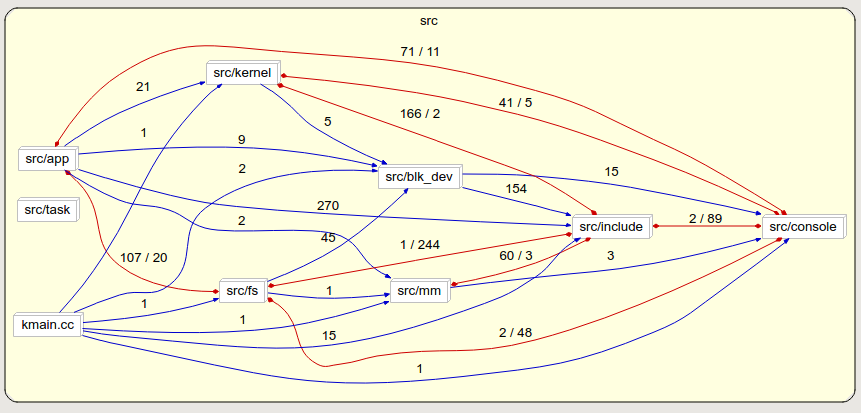
\includegraphics[width=14cm]{pic/assets/dependency_graph}
		\caption{RiOS内核依赖关系图}	\label{dependency_graph}	\end{figure}


目录结构如图~\ref{directory_structure}~所示.	

     \begin{figure}[!htbp]
            \centering	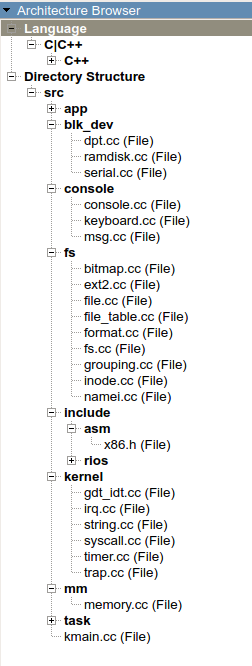
\includegraphics[width=9cm]{pic/assets/directory_structure}
            \caption{目录结构图}	\label{directory_structure}	\end{figure}

\section{系统类图}            

UML类图1如图~\ref{UML_1}~所示.	

     \begin{figure}[!htbp]
            \centering	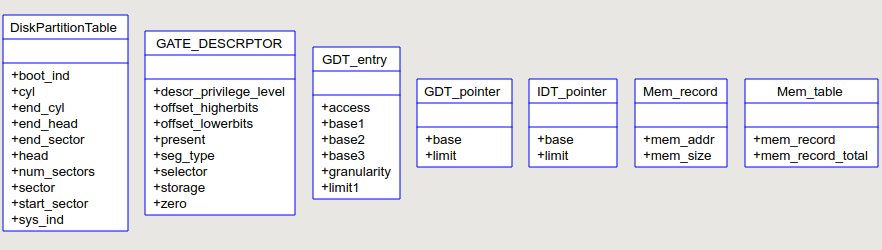
\includegraphics[width=14cm]{pic/assets/UML_1}
            \caption{UML Class Diagram(1) of RiOS kernel}	\label{UML_1}	\end{figure}

UML类图2如图~\ref{UML_2}~所示.	

     \begin{figure}[!htbp]
            \centering	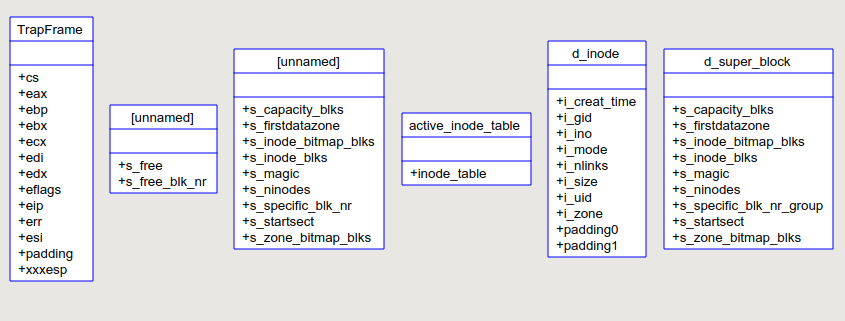
\includegraphics[width=14cm]{pic/assets/UML_2}
            \caption{UML Class Diagram(2) of RiOS kernel}	\label{UML_2}	\end{figure}

UML类图3如图~\ref{UML_3}~所示.	

     \begin{figure}[!htbp]
            \centering	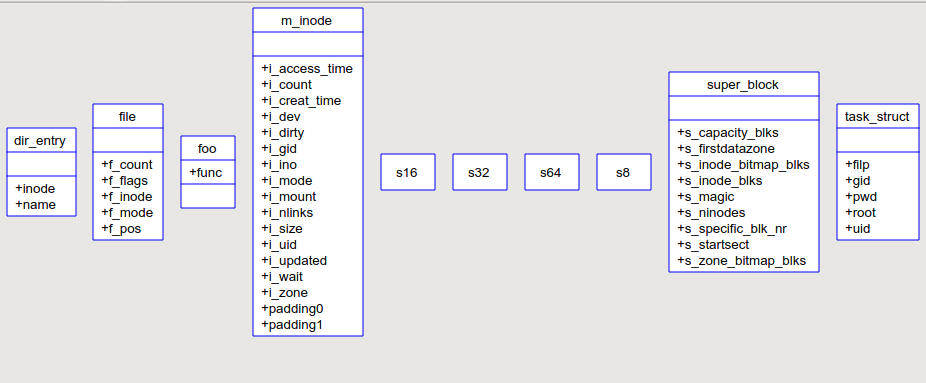
\includegraphics[width=14cm]{pic/assets/UML_3}
            \caption{UML Class Diagram(3) of RiOS kernel}	\label{UML_3}	\end{figure}            

\section{顺序图}
这里展示了开机后做的一系列工作.
顺序图如图~\ref{sequential}~所示.	

     \begin{figure}[!htbp]
            \centering	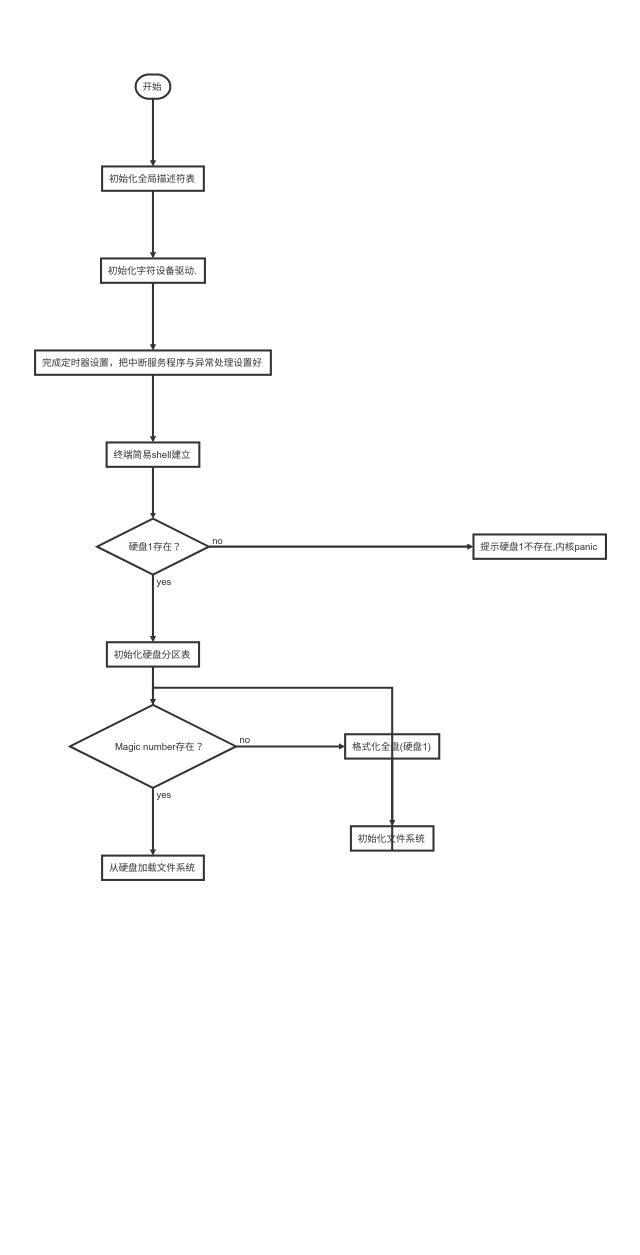
\includegraphics[width=14cm]{pic/assets/sequential}
            \caption{顺序图}	\label{sequential}	\end{figure} 

\section{组成}

\subsection{整体组成}
整体组成如图~\ref{ArchitectureGraph-src}~所示.	

\begin{figure}[!htbp]
       \centering	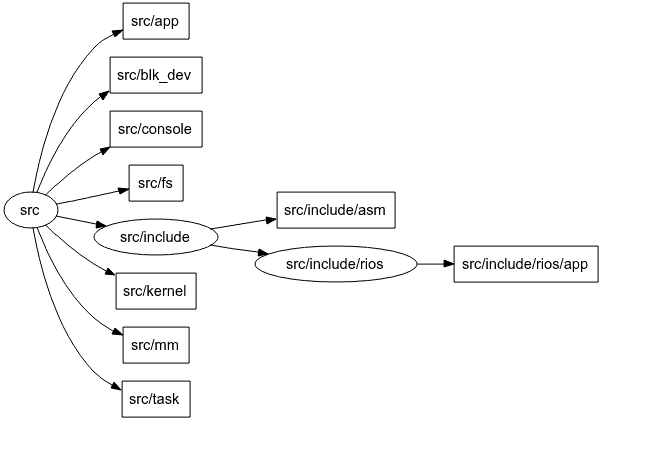
\includegraphics[width=14cm]{pic/assets/ArchitectureGraph-src}
       \caption{ArchitectureGraph-src}	\label{ArchitectureGraph-src}	\end{figure} 

如图~\ref{rios_treemap}~所示.	

     \begin{figure}[!htbp]
            \centering	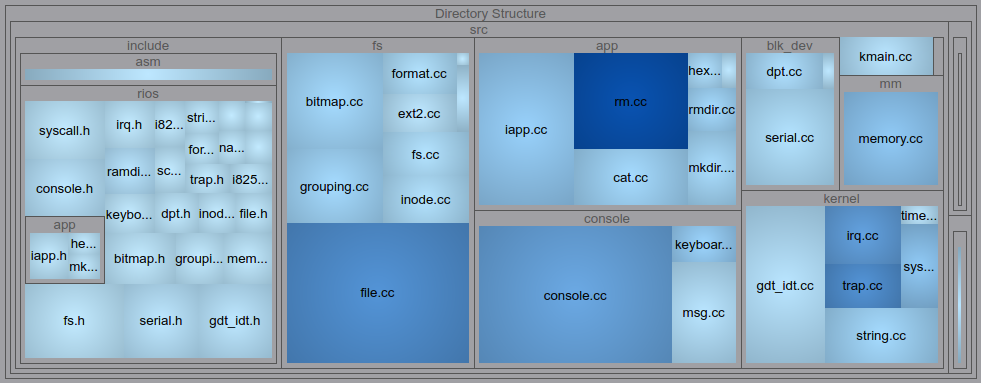
\includegraphics[width=14cm]{pic/assets/rios_treemap}
            \caption{rios treemap}	\label{rios_treemap}	\end{figure} 

\subsection{文件系统组成}
文件系统部分如图~\ref{fs_treemap}~所示.	

     \begin{figure}[!htbp]
            \centering	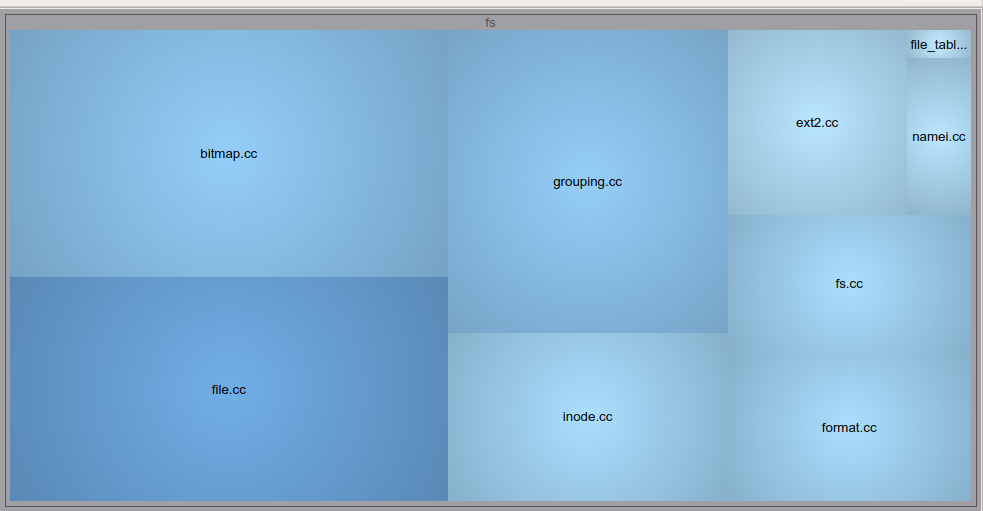
\includegraphics[width=14cm]{pic/assets/fs_treemap}
            \caption{fs treemap}	\label{fs_treemap}	\end{figure} 

\section{依赖关系图}

\subsection{file.cc的依赖关系图}
file.cc依赖关系1如图~\ref{ButterflyGraph-file-cc}~所示.	

     \begin{figure}[!htbp]
            \centering	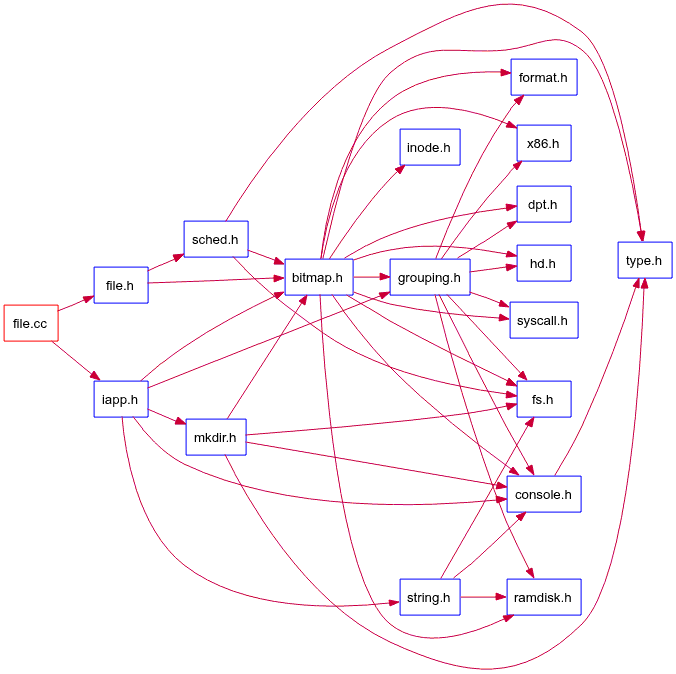
\includegraphics[width=14cm]{pic/assets/ButterflyGraph-file-cc}
            \caption{ButterflyGraph-file-cc}	\label{ButterflyGraph-file-cc}	\end{figure} 
          

\subsection{fs.cc的依赖关系图}
file.cc依赖关系1如图~\ref{ButterflyGraph-fs-cc}~所示.	

     \begin{figure}[!htbp]
            \centering	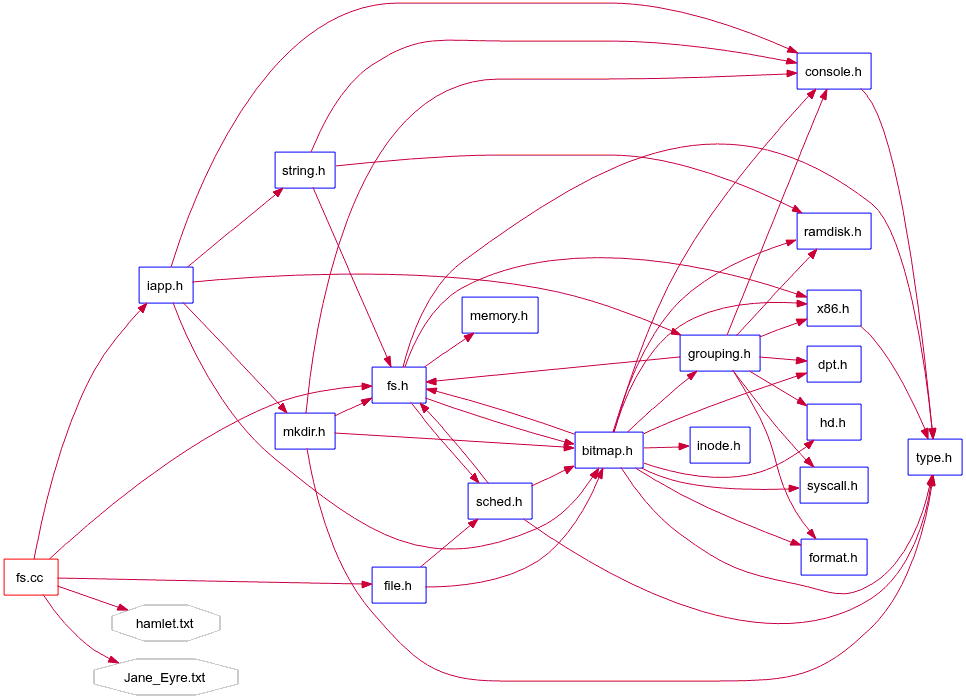
\includegraphics[width=14cm]{pic/assets/ButterflyGraph-fs-cc}
            \caption{ButterflyGraph-fs-cc}	\label{ButterflyGraph-fs-cc}	\end{figure} 

这里只对file.cc和fs.cc两个代码文件依赖关系进行分析,其他可借助understand源代码阅读软件来分析RiOS代码.            

\subsection{整体内部依赖关系图}


整体上,kmain.cc依赖关系1如图~\ref{ButterflyGraph-kmain-cc}~所示.	

     \begin{figure}[!htbp]
            \centering	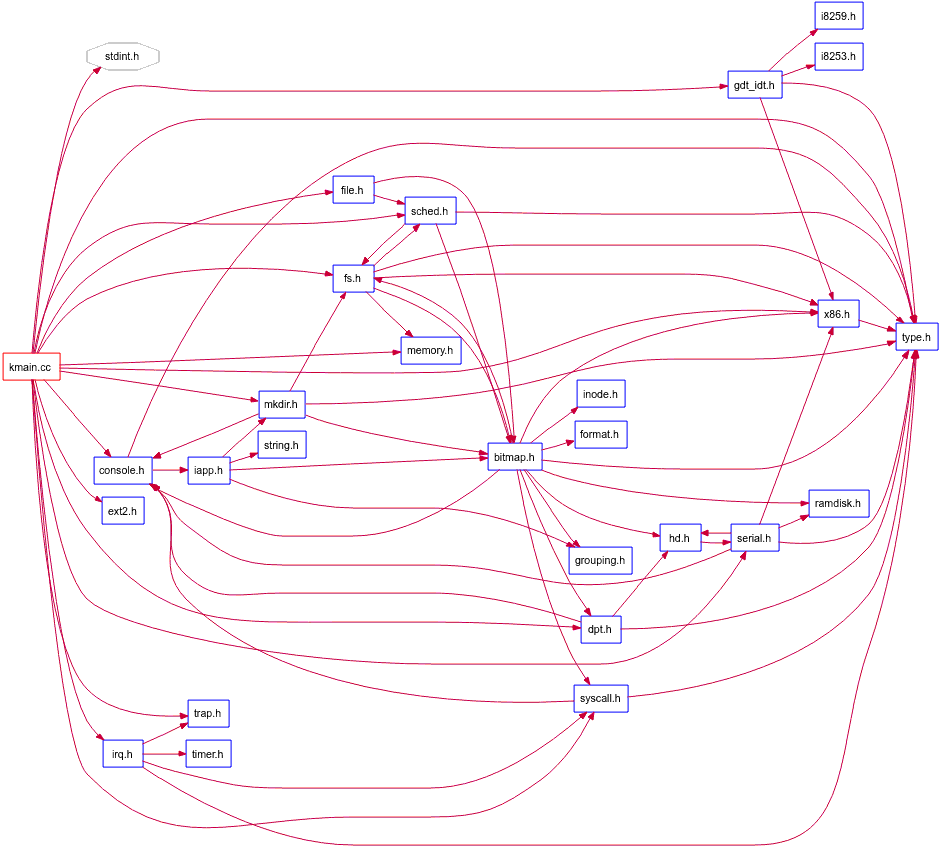
\includegraphics[width=14cm]{pic/assets/ButterflyGraph-kmain-cc}
            \caption{ButterflyGraph-kmain-cc}	\label{ButterflyGraph-kmain-cc}	\end{figure} 


内部依赖图1如图~\ref{ArchInternalDependencies-DirectoryStructure}~所示.	

     \begin{figure}[!htbp]
            \centering	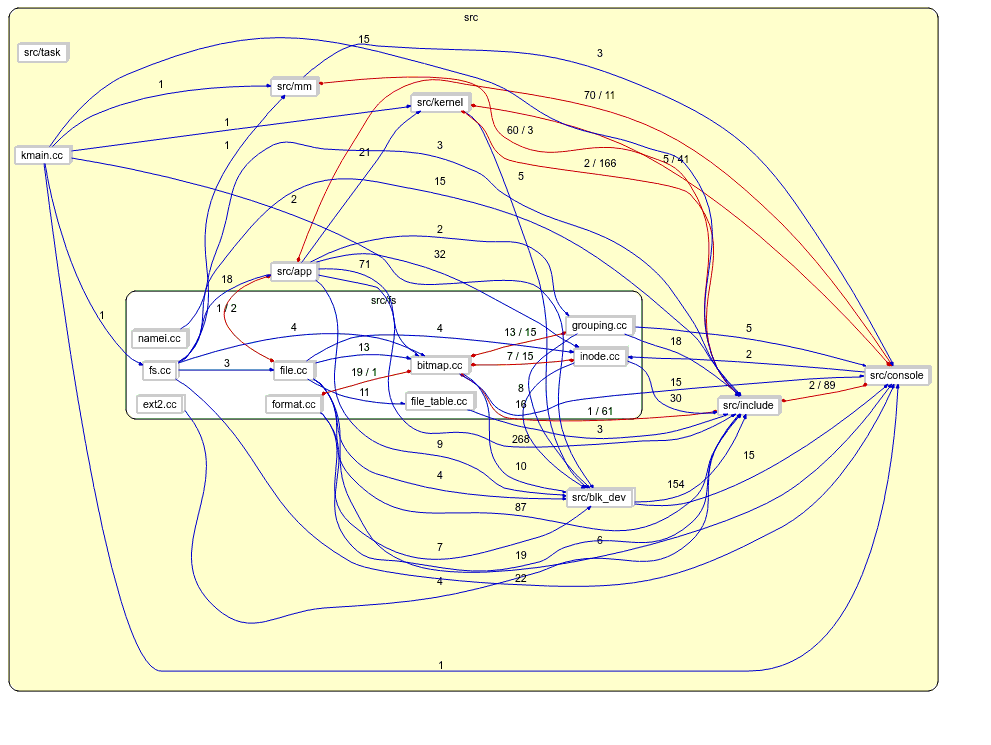
\includegraphics[width=14cm]{pic/assets/ArchInternalDependencies-DirectoryStructure}
            \caption{内部依赖图1}	\label{ArchInternalDependencies-DirectoryStructure}	\end{figure} 

内部依赖图2如图~\ref{ArchInternalDependencies-DirectoryStructure2}~所示.	

     \begin{figure}[!htbp]
            \centering	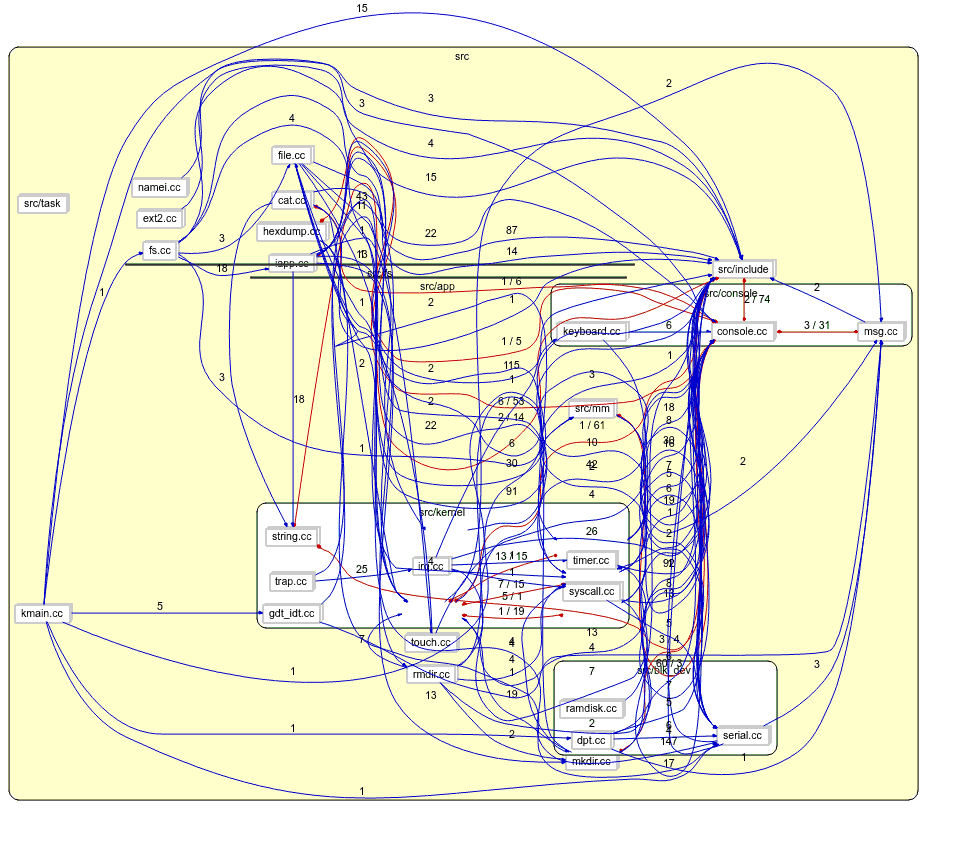
\includegraphics[width=14cm]{pic/assets/ArchInternalDependencies-DirectoryStructure2}
            \caption{内部依赖图2}	\label{ArchInternalDependencies-DirectoryStructure2}	\end{figure} 

内部依赖图3如图~\ref{ArchInternalDependencies-DirectoryStructure3}~所示.	

     \begin{figure}[!htbp]
            \centering	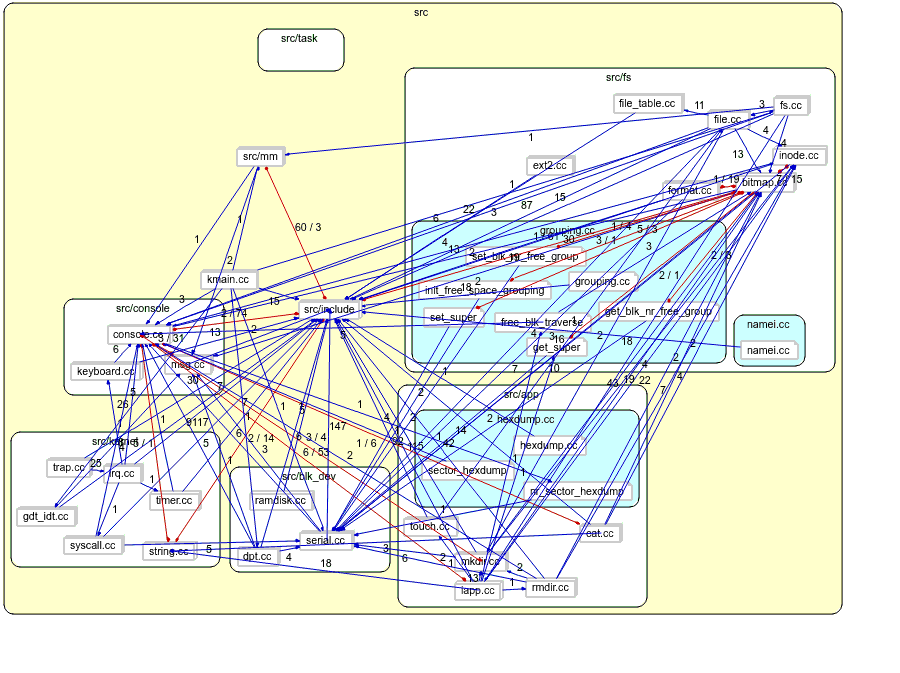
\includegraphics[width=14cm]{pic/assets/ArchInternalDependencies-DirectoryStructure3}
            \caption{内部依赖图3}	\label{ArchInternalDependencies-DirectoryStructure3}	\end{figure} 


% \clearpage